\documentclass[11pt]{article}


\usepackage[margin=1in]{geometry}

\usepackage{mathpazo}

\usepackage{amsmath}

\newcommand{\numpy}{{\sffamily NumPy}}

\usepackage[defaultsans]{cantarell} %% Use option ``defaultsans'' to use cantarell as sans serif only
\usepackage[T1]{fontenc}

% this needs to be done before the fncychap style, since that will 
% redo the chapter stuff
\usepackage{sectsty}
\allsectionsfont{\sffamily}

\usepackage{graphicx}


\begin{document}

\begin{center}
{\bfseries \sffamily \LARGE Making Sense of Power Spectra} \\
Michael Zingale
\end{center}

We are interested in computing the numerical power spectrum of a
function with a known analytic power spectrum, to verify our
algorithm.

Consider a function that is a superposition of sines with different
wavelengths.  The power will be encoded in the amplitude of the sines.
Now imagine this function discretely sampled at $N$ points.  For a domain of
length $L$ the highest possible wavenumber is:
\begin{equation}
k_\mathrm{max} = \frac{1}{\Delta x}
\end{equation}
with $\Delta x = L/N$.  However, for real-valued data, Nyquist sampling
means that $k_\mathrm{max}/2$ is the meaningful maximum.
The lowest wavenumber is:
\begin{equation}
k_\mathrm{min} = \frac{1}{L}
\end{equation}


\section*{\numpy\ details}

The \numpy\ FFTs have the discrete form:
\begin{equation}
\mathcal{F}_k = \sum_{m=0}^{N-1} f_m \exp \left \{ -2\pi i \frac{mk}{N} \right \}
\end{equation}
and the inverse is
\begin{equation}
f_m = \frac{1}{N} \sum_{k=0}^{N-1} \mathcal{F}_k \exp \left \{ 2\pi i \frac{mk}{N} \right \}
\end{equation}
We see from the inverse that if we want to know the amplitude of a single
mode at a given spatial location (denoted by index $m$), that $\mathcal{F}/N$
is the normalized amplitude, i.e., we can think of this expansion as:
\begin{equation}
f_m = \sum_{k=0}^{N-1} \left (\frac{\mathcal{F}_k}{N} \right )
    \exp \left \{ 2\pi i \frac{mk}{N} \right \}
\end{equation}


The {\tt rfftfreq()} function returns the wavenumbers as
\begin{equation}
k = \left \{ 0, \frac{1}{N}, \frac{2}{N}, \ldots, \frac{N-2}{2N}, \frac{1}{2} \right \}
\end{equation}
(for even $n$, and in the mode where we do not specify the sample spacing).
We convert these into a physical quantity (with units of cm$^{-1}$) by
multiplying by $1/\Delta x$, giving the set:
\begin{equation}
k = \left \{ 0, \frac{1}{L}, \frac{2}{L}, \ldots, \frac{1}{2\Delta x} \right \}
\end{equation}

\numpy\ does not have a real-valued FFT function for 3-d data, so we
need to use the {\tt fftn} function.  Because $N$ real numbers results
in $2N$ complex numbers, only 1/2 of the transformed data (in each
dimension) will be unique.  In 3-d this means we consider only an
octant of data.  In practice, this means keeping the positive
frequencies and dropping the negative ones (this is what the {\tt
  rfftfreq} function does for us).




\section*{Power}

For a continuous function, $f(x)$, the ``energy'' is defined as
\begin{equation}
E = \int_{-\infty}^\infty |f(x)|^2 dx
\end{equation}
Using Parseval's theorem, we have
\begin{equation}
E = \int_{-\infty}^\infty |\mathcal{F}(k)|^2 dk
\end{equation}
%
So when we compute the power spectrum, we will be looking at
$|\mathcal{F}(k)|^2$. \\

\noindent [see ``spectral density'' Wikipedia] \\

The discrete version of Parseval's theorem in 1-d is
\begin{equation}
\sum_{n=0}^{N-1} | f(n) |^2 = \frac{1}{N} \sum_{k=0}^{N-1} | \mathcal{F}(k) |^2
\end{equation}
In 3-d, if we have $N^3$ points, then the normalization is $1/N^3$.

\section*{One-dimensional Example}

The idea of the power spectrum is very straightforward in 1-d.  To illustrate
this we will create a function in real space that we expect to have a
power spectrum scaling as:
\begin{equation}
P \sim k^{-\eta}
\end{equation}
This is accomplished by setting the amplitude of each mode to yield
this power.  Our function is:
\begin{equation}
f(x) = \sum_{m=1}^{N_\mathrm{modes}} a_m \sin \left ( \frac{2\pi m x}{L}\right )
\end{equation}
where $L$ is the width of the physical domain, and 
\begin{equation}
a_m = \left (A_0 k^{-\eta} \right )^{1/2}
\end{equation}
This function is shown in Figure~\ref{fig:phi1d}.

\begin{figure}[t]
\centering
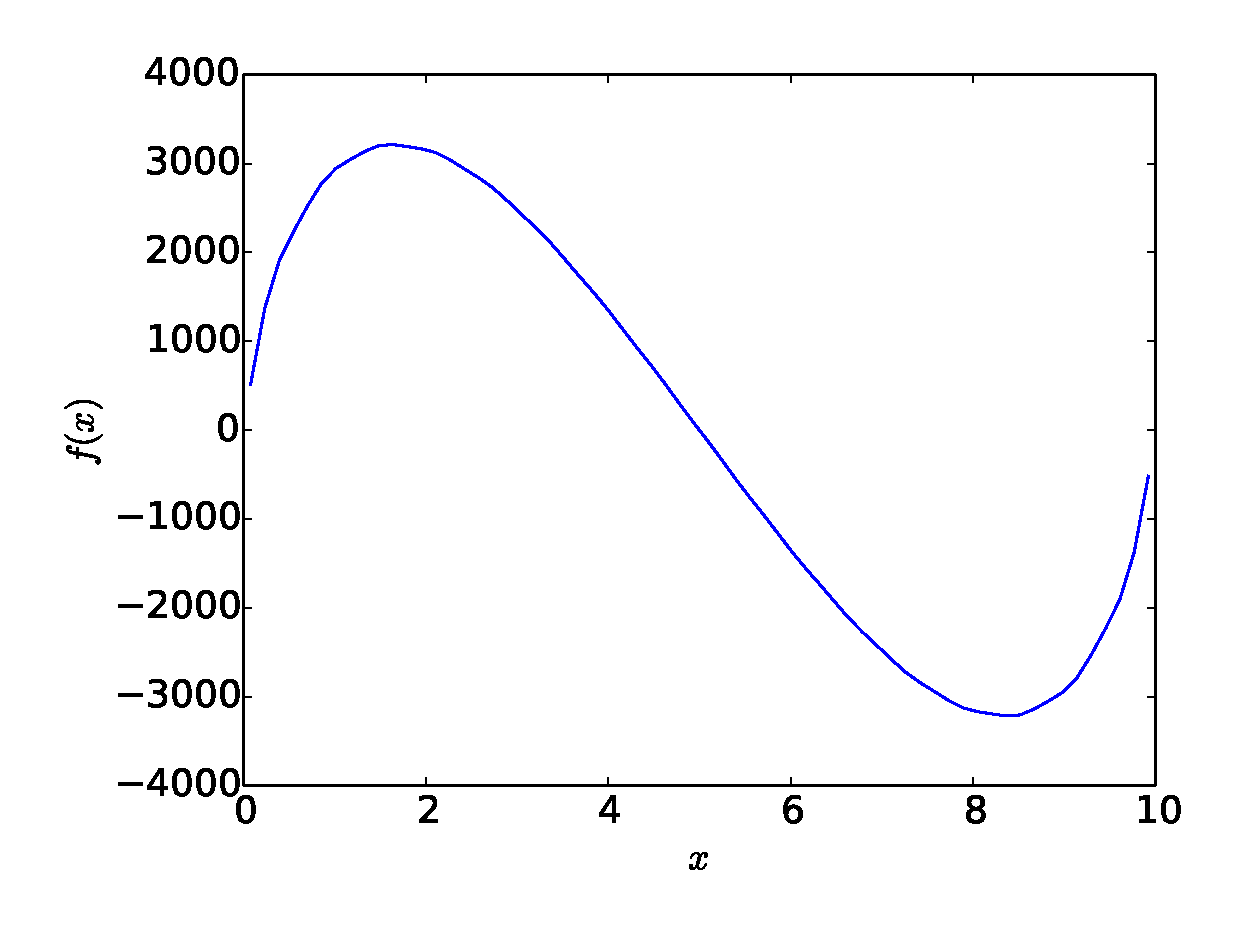
\includegraphics[width=0.5\linewidth]{phi_1d}
\begin{minipage}[b]{0.45\linewidth}
\caption{\label{fig:phi1d} The real-space, one-dimensional function $f(x)$.}
\end{minipage}
\end{figure}

We then transform this function, denoting the transform as $\mathcal{F}(k)$.  Plotting
$|\mathcal{F}(k)|^2$ vs.\ $k$ gives the power spectrum.  Figure~\ref{fig:ps1d} shows
the result, together with the expected power-law scaling, $P$, shown as the 
dashed line.

\begin{figure}[t]
\centering
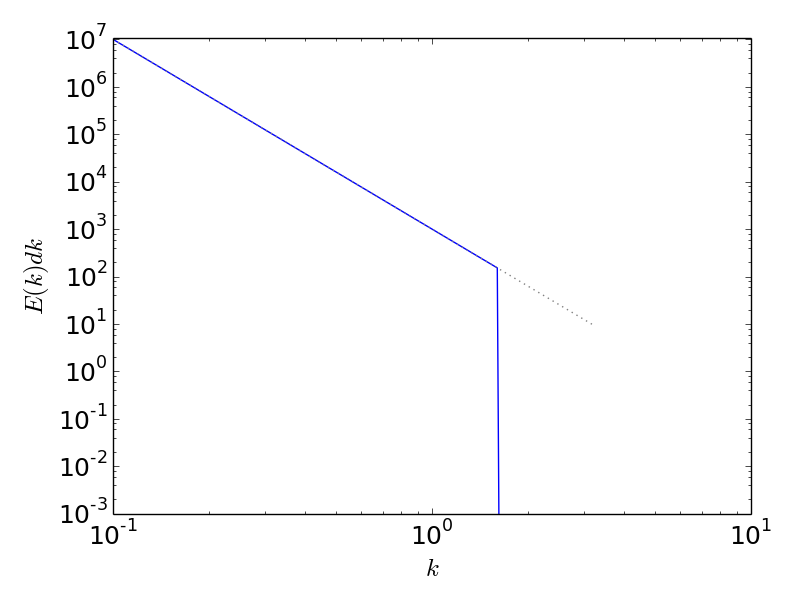
\includegraphics[width=0.5\linewidth]{ps1d}
\begin{minipage}[b]{0.45\linewidth}
\caption{\label{fig:ps1d} The power spectrum of $f(x)$.}
\end{minipage}
\end{figure}



See {\tt ps1d.py} for the implementation of this test.



\section*{Three-dimensional Case}

In 3-d, things are more complex---we will need to bin the transformed
function in spherical shells corresponding to our discrete $k$.  The
power spectrum is defined as
\begin{equation}
E(k) = \frac{1}{\Omega} \int_{S(k)} \mathcal{F}(k) \mathcal{F}^\star(k) dS
\end{equation}
where $\Omega$ is the volume in physical space, and the integral is done
over the space $S(k)$, the surface defined by $|\vec{k}| = k$.  We can
write $dS = 4\pi k^2 dk$ and integrate along radial $|\vec{k}|$.


Again, to test the algorithm, we define a test function and set the power at
different wavenumbers {\em in physical space}, and then do the transform
and power spectrum to see if we get the expected result.  We will design
our function to have the same scaling as the 1-d case, $P \sim k^{-\eta}$.
Our test function
is:
\begin{equation}
\phi(x,y,z) = \sum_{m=1}^{N_\mathrm{modes}} 
              \sum_{n=1}^{N_\mathrm{modes}} 
              \sum_{p=1}^{N_\mathrm{modes}} 
     a_{m,n,p} \sin \left ( \frac{2\pi m x}{L_x} + 
                            \frac{2\pi n y}{L_y} + 
                            \frac{2\pi p z}{L_z} \right )
\end{equation}
where we can identify the wavenumbers in each direction as
\begin{equation}
k_m = \frac{m}{L_x} \, ; \quad 
k_n = \frac{n}{L_y} \, ; \quad 
k_p = \frac{p}{L_z} \,
\end{equation}
This is equivalent to defining a vector wavenumber
\begin{equation}
\vec{k} = k_m \hat{x} + k_n \hat{y} + k_p \hat{z}
\end{equation}
and expressing a single component as
\begin{equation}
\phi_{m,n,p} = a_{m,n,p} \sin(2\pi \vec{k}\cdot \vec{x})
\end{equation}


In discrete form, we bin the $k$ in our transformed space into a
number of uniformly spaced bins, $\kappa_l$, where the index
$l$ denote the bin boundaries, with $\kappa_0$ the leftmost bin boundary.
Our power spectrum becomes
\begin{equation}
E(\kappa_l) = \sum_{\kappa_{l-1} \le |\vec{k}| < \kappa_l} \mathcal{F}(k) \mathcal{F}^\star(k)
\end{equation}
where the sum is over all the zones in the $k_x \times k_y \times k_z$ cube
whose wavenumber magnitude, $k$, falls into our bin.  As we go to
higher wavenumbers, the number of zones will increase as $k**2$---this
captures the $dS$ scaling in the continuous-form of the power spectrum.

We can set the amplitude of component based on our desired
powerlaw scaling.  Defining $k = |k|$, and $A_0$ as a
reference amplitude of the power, we take
\begin{equation}
a_{m,n,p}^2 = \frac{A_0 k^{-\eta}}{W(k)} \frac{1}{4\pi k^2}
\end{equation}
where $W(k)$ is the weight that accounts for the fact that multiple
combinations of $m, n, p$ can result in the same $k$.  Using Iverson bracket
notation, defined as
\begin{equation}
[P] = \begin{cases}
  1 & \text{if P is true} \\
  0 & \text{otherwise}
      \end{cases}
\end{equation}
we find $W(k)$ as
\begin{equation}
W(k) = \sum_{m=1}^{N_\mathrm{modes}}
       \sum_{n=1}^{N_\mathrm{modes}} 
       \sum_{p=1}^{N_\mathrm{modes}} [ k_m^2 + k_n^2 + k_p^2 = k ]
\end{equation}
The factor $4\pi k^2$ in the denominator reflects the $dS$ in the 
definition of the power spectrum integral.

\end{document}
